\chapter{Statistical Models and Identifiability}
\label{ch:models}

\begin{chaptergoals}
\begin{itemize}[nosep]
\item What a statistical model is: a sample space and a family of candidate distributions indexed by a parameter. The whole of the rest of the book happens inside this object.
\item The chain from the abstract sample space to the numbers in the data file, walked once for the kiss experiment: outcomes, random variables as functions on them, and observations as those functions evaluated at the outcome that happened.
\item The trade that modeling always makes: assumptions buy fewer parameters to learn, at the price of being wrong if the assumptions are. The siblings example, drawn both ways.
\item Well-specified models, and parametric versus nonparametric ones.
\item Identifiability: when the distribution of the data pins down the parameter, and when it doesn't, with the standard example drawn in the parameter space so you can see what fails.
\item Gaussian mixture models, as a generative story and as an example of a model whose parameter is identifiable only up to relabeling.
\end{itemize}
\Cref{ch:kiss} made three assumptions about the kiss experiment and called the result a model. This chapter says what a model is in general, so that everything from Part III on can be stated for any model and not only the Bernoulli one.
\end{chaptergoals}

\section{The rationale behind statistical modeling}
\label{sec:models-rationale}

\Cref{ch:kiss} was about one estimator, $\hat{p} = \bar{R}_n$, under one set of assumptions.
To say what estimators, intervals and tests are in general, you first have to fix the object they all live in: a model, which is the three assumptions of \cref{sec:kiss-assumptions} written as a mathematical object.
The rationale behind statistical modeling can be outlined as follows:
\begin{itemize}
\item Let $\Xton$ be $n$ independent copies of $X$.
The goal of statistics is to learn the distribution of $X$.

\textbf{NB:} It's crucial to understand this notation, this way of specifying problems, and, most importantly, the relationship between the $n$ i.i.d.\ r.v.s $\Xton$ and the r.v.\ $X$.
Each of the $n$ i.i.d.\ r.v.s $\Xton$ has the same distribution as the r.v.\ $X$.
The relationship between $X$ and $\Xton$ can be understood as follows:
\begin{enumerate}[nosep]
\item $X$ is the underlying r.v.\ of interest, with an unknown distribution that you want to learn.
\item $\Xton$ are $n$ r.v.s that form your sample of observations drawn from the same distribution as $X$.
This is all-important: When you see something like `Suppose $\Xton$ are $n$ independent copies of $X$' you should \textit{automatically interpret these $n$ variables as your sample data}.
\end{enumerate}
By observing the values of $\Xton$, you can make inferences about the distribution of $X$.

\item If $X \in \{0,1\}$, then it's Bernoulli and you only have to learn the parameter $p$.
That was the kiss experiment.

\item It can be more complicated.
Take a (partial) dataset of the number of siblings, including self, collected from college students:
\[
2, 3, 2, 4, 1, 3, 1, 1, 1, 1, 1, 2, 2, 3, 2, 2, 2, 3, 2, 1, 3, 1, 2, 3, \ldots
\]
If $X \in \{1, 2, 3, 4, 5, 6, \geq 7\}$, each with a different probability $\Pr(X = x)$, then you could make no assumption and try to learn the whole PMF: that's $7$ parameters to learn (six, really, since they sum to one).

\item Or you could assume that $X - 1 \sim \Pois(\lambda)$.
That's only 1 parameter, $\lambda$, to learn.
\Cref{fig:siblings} shows both on the siblings data.
The empirical PMF is seven numbers, six of them free since they sum to one; the model is one number, $\hat\lambda$, set to the sample mean minus one.
The model fits well here; where such a model didn't fit, the fault would be the assumption's, not the data's.

\item \textbf{NB:} It's important to keep in mind that parameters define distributions.
What is meant is that, suppose you're considering the family of Gaussian distributions.
Once you specify $\mu$ and $\sigma^2$, you've fixed the distribution.
Learning the parameter and learning the distribution are the same task.
(The Gaussian family appears in several examples of this chapter, written $\Gauss(\mu, \sigma^2)$ with the variance second, and with $\Phi$ for the CDF of $\Gauss(0,1)$; \cref{ch:gaussian} is its full treatment, and the notation page has what is needed here.)
\end{itemize}

\begin{figure}[htbp]
\centering
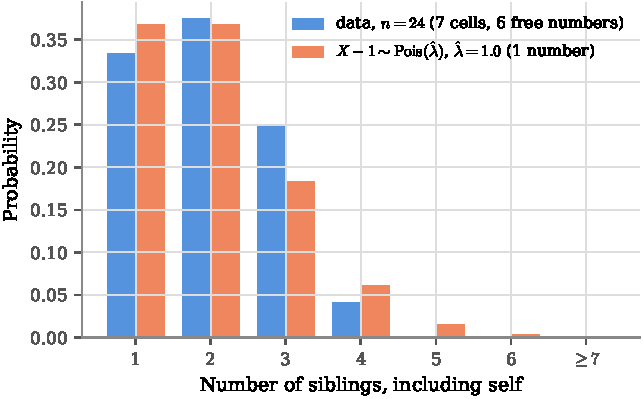
\includegraphics[width=0.78\textwidth]{fig_siblings_model}
\caption{The siblings data ($n = 24$ values) as an empirical PMF (blue), next to the fitted one-parameter model $X - 1 \sim \Pois(\hat\lambda)$ (orange), with $\hat\lambda$ the sample mean minus one.}
\label{fig:siblings}
\end{figure}

\begin{intuition}[assumptions are currency]
Every assumption you add to a model buys you something and costs you something.
`$X - 1$ is Poisson' reduces seven unknowns to one, which means $24$ observations go a long way instead of being spread over seven cells, and it lets you say things about families of $8$ siblings that you never observed.
What it costs is the possibility of being wrong: if the real PMF isn't Poisson-shaped, no amount of data will make the model right, and the estimate of $\lambda$ will be a precise estimate of the wrong thing.
The phrase for this is that a model should be plausible, and the mathematics that follows assumes it is.
Checking the assumption is the job of the goodness-of-fit tests in \cref{ch:gof}.
\end{intuition}

\section{Statistical models}
\label{sec:models-definition}

\begin{definition}[Statistical model]
\label{def:statmodel}
Let the observed outcome of a statistical experiment be a sample $\Xton$ of $n$ i.i.d.\ r.v.s in some sample space $E$ (usually $E \subseteq \real$; the requirement that $E$ be measurable is a technicality, see \toolkit{sec:math-rv}) and denote by $\Pr$ their common distribution.
A \textbf{statistical model} associated to that statistical experiment is a pair:
\[
\left(E, (\Pr_\theta)_{\theta \in \Theta} \right),
\]
where:
\begin{itemize}[nosep]
\item $E$ is the \textbf{sample space} for $X$; that is, the set containing all possible outcomes of $X$.
The sample space is therefore also where your observations, $\Xton$, live.
\item $(\Pr_{\theta})_{\theta \in \Theta}$ is a family of probability distributions on $E$, the candidate distributions for $X$.
\item $\Theta$ is the \textbf{parameter space}; that is, a set consisting of the possible values of $\theta$.
\end{itemize}
\end{definition}

\begin{inwords}
\textbf{In words.} A model is a list of candidate explanations for the data: where an observation can land ($E$), and every distribution you are willing to consider as the one that produced it, with a label $\theta$ on each.
\par\smallskip
\textbf{For the kiss data.} $E = \{0, 1\}$, the candidates are the $\Bern(p)$ distributions, one for each $p \in (0,1)$, and the label is $p$ itself. `Learn the model' means `find out which label is right'.
\end{inwords}

\textbf{Note:} A \textbf{probability measure} or \textbf{probability distribution} takes an event $A \subseteq E$ as input and returns $\Pr_\theta(A)$ \toolkit{sec:math-rv}.
It is assumed to satisfy the usual axioms of probability.
Most importantly, a probability measure is not a PMF or PDF.
A probability measure assigns probabilities to events in the sample space, while a PMF or PDF assigns probabilities (or densities) to specific values of a discrete or continuous r.v.
The two determine each other, so in practice you write down the family by writing down its PMFs or PDFs, as in the examples below, but the object in the definition is the distribution.

\Cref{fig:modelfamilies} is the picture to keep in mind: a model is a family of distributions, and the parameter is the label that picks one out.
In the top row, two one-parameter families; sliding the parameter moves you through the family.
In the bottom row, the Gaussian family has a two-dimensional parameter space, drawn on the left, and each point of it is one distribution, drawn on the right.
The arrow $\theta \mapsto \Pr_\theta$ from the left of the figure to the right is what the definition is about, and \cref{sec:models-identifiability} asks whether it ever sends two points to the same distribution.

\begin{figure}[htbp]
\centering
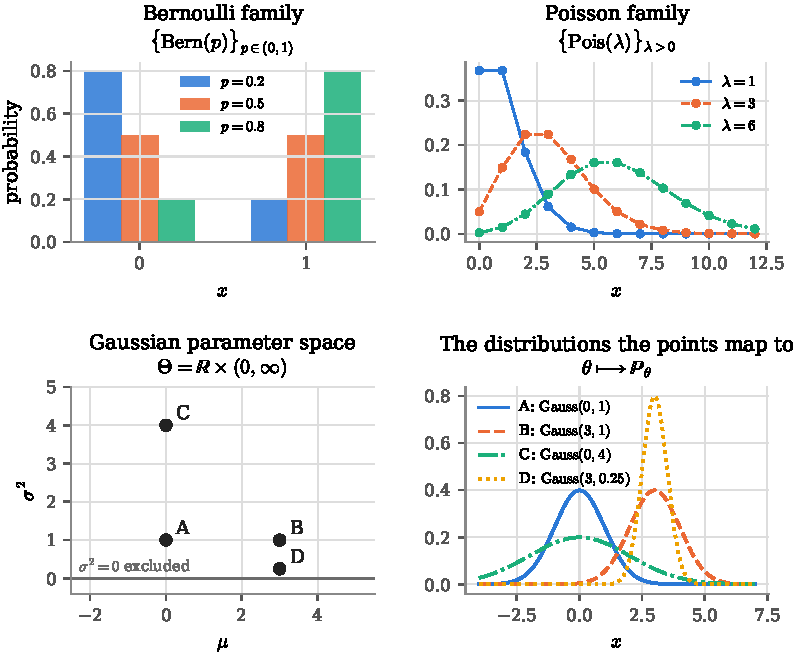
\includegraphics[width=\textwidth]{fig_model_families}
\caption{Top: the Bernoulli family at three values of $p$, and the Poisson family at three values of $\lambda$. Bottom: four points A to D in the Gaussian parameter space $(\mu, \sigma^2)$, left, and the densities they map to, right.}
\label{fig:modelfamilies}
\end{figure}

\subsection{Examples of parametric models}

For parametric models (defined in \cref{sec:models-parametric}: the parameter is a list of finitely many numbers), the parameters live in some space that's a subset of $\real^d$ and the parameters can be represented by a vector.
Here are some canonical examples of parametric models:
\begin{enumerate}
\item For $n$ Bernoulli trials: $\left( \{0, 1\}, (\Bern(p))_{p \in (0,1)} \right)$.
The vectors of parameters thus consist of singletons $(p)$.

\item If $\Xton \iid \Pois(\lambda)$ for some unknown $\lambda > 0$: $\left( \mathbb{N}, (\Pois(\lambda))_{\lambda > 0} \right)$.
The vectors of parameters thus consist of singletons $(\lambda)$.

\item If $\Xton \iid \Gauss(\mu, \sigma^2)$ for some unknown $\mu \in \real$ and $\sigma^2 > 0$:
\[
\left( \real, (\Gauss(\mu, \sigma^2))_{(\mu, \sigma^2) \in \real \times (0, \infty)} \right).
\]
The vector of parameters has length 2 and is given by $(\mu, \sigma^2)$.

\item If $\Xton \iid \Gauss_d(\mu, \ident_d)$ for some unknown $\mu \in \real^d$: $\left( \real^d, (\Gauss_d(\mu, \ident_d))_{\mu \in \real^d} \right)$.
The vector of parameters is $\mu$ itself, of length $d$.

\item If $\Xton \iid \text{Unif}([0, a])$ for some unknown $a > 0$: $\left( \real_+, (\text{Unif}([0, a]))_{a > 0} \right)$.
Not $\left( [0, a], \ldots \right)$: see the pitfall below.
\end{enumerate}

Sometimes there's no simple notation like $\Bern(p)$ for the family and you have to be more explicit.
The linear regression model: $(X_1, Y_1), \ldots, (X_n, Y_n) \in \real^d \times \real$ are i.i.d.\ with $Y_i = \beta^\top X_i + \epsilon_i$, $\epsilon_i \iid \Gauss(0,1)$ independent of $X_i \sim \Gauss_d(0, \ident_d)$, for an unknown $\beta \in \real^d$.
Here $E = \real^d \times \real$, $\Theta = \real^d$, and $\Pr_\beta$ is the joint distribution of the pair $(X, Y)$ that this recipe produces.
\Cref{ch:regression-multi} is about this model in a slightly different form: the $X_i$ treated as fixed numbers rather than Gaussian draws, and the error variance $\sigma^2$ unknown, which makes $\Theta = \real^d \times (0, \infty)$ and makes the $Y_i$ independent but no longer identically distributed, since each has its own mean $\beta^\top x_i$.
Treating the predictors as fixed is what lets the regression chapter condition on them and still have a model in the sense of \cref{def:statmodel}.

\begin{pitfall}[the sample space must not depend on the parameter]
Which of these is a statistical model for $n$ Bernoulli trials: $\left( \{1\}, (\Bern(p))_{p \in (0,1)} \right)$ or $\left( \{0,1\}, (\Bern(p))_{p \in (0.2, 0.4)} \right)$?
Only the second.
The first has a sample space that leaves out an outcome the distributions put mass on; a Bernoulli r.v.\ takes the value $0$, so $\{1\}$ isn't where the observations live.
The second is a model, just one that assumes $p$ is between $0.2$ and $0.4$ (which may or may not be well-specified, the next section's question).
Similarly, for $\Xton \iid \text{Unif}([0, a])$ with $a$ unknown, the model is $\left( \real_+, (\text{Unif}([0, a]))_{a > 0} \right)$ and not $\left( [0, a], \ldots \right)$: the sample space is fixed before you know $a$, so it has to be a set that contains every observation for every candidate $a$.
Any such set will do ($\real$ works too); the convention in this book is the smallest natural one.
A sample space that mentions the unknown parameter is not a sample space.
\end{pitfall}

\begin{bridge}[the model was always there]
In an introductory course the model is a sentence: `assume the data are normally distributed', `assume each trial succeeds with the same probability'.
This book makes the sentence into an object with three parts, and the point of doing so is that every later statement can name exactly what it depends on.
`The sample mean is unbiased' is a statement about $\E_\theta[\bar{X}_n]$ for every $\theta \in \Theta$; `the $t$-test has level $5\%$' is a statement that holds for every member of the Gaussian family; `the estimator is consistent' means $\hat{\theta}_n \to \theta$ under $\Pr_\theta$ for every $\theta$.
When a method fails in practice, it is often because the data came from outside the family, and you can only say that if the family is written down.
\end{bridge}

\section{From the sample space to the data and back}
\label{sec:models-sample-space}

The definition says the observations live in a sample space $E$, and a random variable is, by definition, a function on a sample space $S$ \toolkit{sec:math-rv}; \cref{ch:lln} returns to that definition when it needs sequences of random variables.
These are two uses of the same phrase for two different sets, and the gap between them is where the single most common confusion in this subject lives: what is the relationship between the abstract space on which probability is defined and the concrete numbers in the data file?
This section walks the chain once, slowly, for the kiss experiment, with \cref{fig:layers} as the map.
On the left of the figure is the sample space $\Omega$, one point per complete possible outcome of the study, with the one that happened marked.
In the middle, the data are a function on $\Omega$, one row of $0$s and $1$s per outcome, and the marked row is the data set you have.
On the right, the statistic $\bar R_n$ is another function on $\Omega$; over all outcomes weighted by their probabilities it has a distribution, the bars, and the marked outcome gives the one value you observe, $\bar r_n = 8/12$.
Nothing travels from right to left: the dashed arrow is inference, which holds the one value up against the distribution of the rule.

\begin{figure}[htbp]
\centering
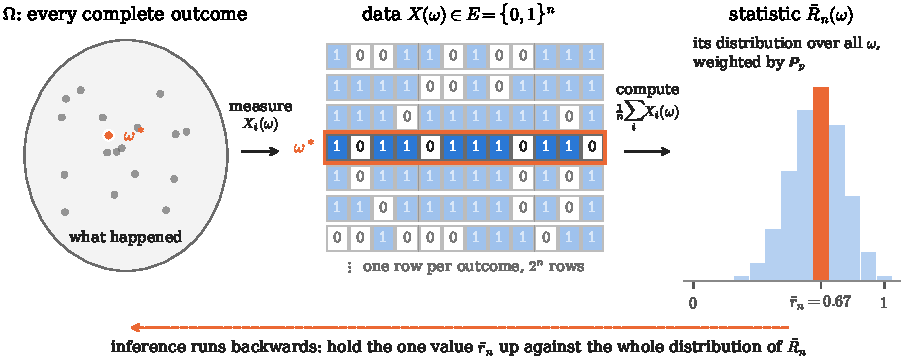
\includegraphics[width=\textwidth]{fig_sample_space_layers}
\caption{The sample space $\Omega$ (left), the data as one row of $0$s and $1$s per outcome (middle), and the statistic $\bar R_n$ with its distribution (right), for a kiss experiment with $n = 12$. The outcome that happened is marked in orange.}
\label{fig:layers}
\end{figure}

\textbf{Layer one: the sample space.}
An outcome $\omega$ of the study is everything that could happen, in full detail: which $124$ couples were observed, where and in which order, and which way each one turned.
The set of all such outcomes is the sample space, written $\Omega$ here ($S$ in the toolkit and in \cref{ch:lln}).
It is as abstract as the subject gets, and you never see an element of it.
What you see is what your measuring instruments report about the one $\omega$ that occurred.

\textbf{Layer two: random variables are the measuring instruments.}
A random variable is a function on $\Omega$ \toolkit{sec:math-rv}.
The instrument for couple $i$ is $R_i$, with $R_i(\omega) = 1$ if, in outcome $\omega$, couple $i$ turned right and $0$ otherwise.
The data vector $(R_1, \ldots, R_n)$ is a function on $\Omega$ too, with values in $E^n = \{0,1\}^n$; one row of \cref{fig:layers} per outcome.
And $\bar{R}_n = \frac{1}{n}\sum_i R_i$ is yet another function on $\Omega$.
That is all `the estimator is a random variable' means: a rule that could be applied to any outcome, written down before you know which outcome you will get.

\textbf{Layer three: the observations are those functions evaluated at the outcome that happened.}
Nature picked one $\omega^*$.
Your data are $r_1 = R_1(\omega^*), \ldots, r_n = R_n(\omega^*)$, and your estimate is $\bar{r}_n = \bar{R}_n(\omega^*) = 0.645$.
Going from the sample space to the observations is `plug in the $\omega$ that occurred'.
A realization is one evaluation of a function; a distribution is how often each value would come up across all of $\Omega$, weighted by probability.
The realized number $0.645$ is one draw from the distribution of $\bar{R}_n$; after it is observed it is a fixed number, and the distribution belongs to the rule, not to the number (the pitfall in \cref{sec:kiss-test}).

\textbf{Going back is not an inverse.}
You never recover $\omega^*$ from the data, and you do not need to.
What inference does instead is ask, for each candidate $\theta$: across all the outcomes that could have occurred under $\Pr_\theta$, how often would $\bar{R}_n$ have landed near the value it took?
The one number is held up against the whole distribution of the rule, and the candidates under which it would have been typical are the plausible ones.
That is the dashed arrow in \cref{fig:layers}, and it is what every confidence interval and test in this book does.

\begin{intuition}[the trick that makes $\Omega$ concrete]
Since $\Omega$ only ever enters through the random variables defined on it, you may as well take $\Omega$ to be the set of data sets you could have gotten.
For the kiss experiment that is $\Omega = \{0,1\}^{124}$, a finite set with $2^{124}$ elements, and under the model $\Pr_p(\omega) = p^{\#\text{ones}}(1-p)^{\#\text{zeros}}$.
Every row of \cref{fig:layers} is a point of this $\Omega$, and $R_i(\omega)$ is just `the $i$-th entry of the row'.
This is why \cref{def:statmodel} mentions $E$ and never $\Omega$: for a fixed $n$ the observable sample space $E^n$ \textit{is} the sample space, and a model is a family of probabilities on it.
The abstract $\Omega$ of probability theory is needed only when one space has to carry infinitely many random variables at once, $R_1, R_2, R_3, \ldots$ without end, which is exactly what the limit theorems of Part II need in order to say `as $n \to \infty$'.
For any fixed $n$, think $\Omega = E^n$ and nothing is lost.
\end{intuition}

\begin{bridge}[the sampling distribution, defined rather than simulated]
An introductory course introduces the sampling distribution of the sample mean by rerunning the study: draw many samples, compute $\bar{x}$ for each, draw the histogram.
That histogram is the right of \cref{fig:layers}, approximated by simulation; this chapter defines it instead, without rerunning anything, by putting a probability on $\Omega$ and asking how $\bar{R}_n(\omega)$ is distributed under it.
The two pictures agree: each simulated sample is one $\omega$, an introductory course's `many samples' are many points of $\Omega$, and the limit of the histogram as the number of samples grows is the distribution of the random variable.
\Cref{fig:twoaverages} in \cref{ch:lln} draws the same picture as rows and columns: a row is an $\omega$, the row average is $\bar{R}_n(\omega)$, and the column of row averages is the sampling distribution.
Your data set is the one row nature handed you.
\end{bridge}

\section{Well-specified models}
\label{sec:models-wellspecified}

It is almost always assumed that a statistical model is well-specified.

\begin{definition}[Well-specified]
\label{def:wellspecified}
A model $\left(E, (\Pr_\theta)_{\theta \in \Theta }\right)$ is \textbf{well-specified} if there exists some $\theta \in \Theta$ such that $\Pr = \Pr_{\theta}$, where $\Pr$ is the true distribution that generates the observed data $\Xton$.
In other words, $\Pr \in (\Pr_{\theta})_{\theta \in \Theta}$.
If $\Pr \notin (\Pr_{\theta})_{\theta \in \Theta}$, then the model is \textbf{misspecified}.
That particular $\theta$ such that $\Pr = \Pr_{\theta}$ is the \textbf{true parameter}, often written $\theta^*$, and is unknown.
\end{definition}

\begin{inwords}
\textbf{In words.} The true distribution is on your list of candidates. If it isn't, no label is right, and `the true parameter' has no meaning.
\par\smallskip
\textbf{For the kiss data.} If couples really do turn right with a single probability $p^*$, independently, the model is well-specified and $p^* \in (0,1)$ is the true parameter. If, say, the probability differed by country, no single $\Bern(p)$ reproduces the data-generating process and the model is misspecified.
\end{inwords}

\begin{center}
\begin{tikzpicture}[font=\small]
  \begin{scope}
    \draw[rounded corners=8pt, fill=boxblue!6, draw=boxblue!60!black] (0,0) rectangle (3.6,2.2);
    \node[anchor=north west, font=\scriptsize] at (0.1,2.15) {$(\Pr_\theta)_{\theta\in\Theta}$};
    \fill[boxaqua!70!black] (2.1,1.0) circle (2.2pt) node[right=1pt, font=\scriptsize] {$\Pr = \Pr_{\theta^*}$};
    \node[below, font=\scriptsize] at (1.8,-0.05) {well-specified: the truth is in the family};
  \end{scope}
  \begin{scope}[xshift=5.2cm]
    \draw[rounded corners=8pt, fill=boxblue!6, draw=boxblue!60!black] (0,0) rectangle (3.6,2.2);
    \node[anchor=north west, font=\scriptsize] at (0.1,2.15) {$(\Pr_\theta)_{\theta\in\Theta}$};
    \fill[boxorange!80!black] (4.3,1.0) circle (2.2pt) node[right=1pt, font=\scriptsize] {$\Pr$};
    \node[below, font=\scriptsize] at (2.3,-0.05) {misspecified: no $\theta$ reproduces the truth};
  \end{scope}
\end{tikzpicture}
\end{center}

Here's an example to illustrate the meaning of well-specified models:
\begin{itemize}
\item Suppose you're modeling the outcome of a coin toss using a Bernoulli distribution with parameter $p$, where $p$ represents the probability of getting heads.
Suppose further that the \textit{true} probability of getting heads is $p^* = 0.6$.
\item Now, if your model considers all possible values of $p \in (0,1)$, then it's a well-specified model because it includes the true probability distribution, the $\Bern(0.6)$ distribution, as one of the possible distributions in the family.
\item On the other hand, if your model only considers values of $p$ between, say, 0 and 0.5, then it's not well-specified because it doesn't include the true probability distribution, $\Bern(0.6)$, in the family of distributions.
\end{itemize}

The above example addresses misspecification when the true parameter value is not contained in your model's parameter space.
But a model misspecification could also be due to applying the `wrong' distribution: for example, by modeling the toss of a coin using a Gaussian distribution, or the siblings data of \cref{fig:siblings} with a shifted Poisson when the true PMF has a second bump at $5$.

One aim of a statistical experiment is to \textit{estimate} the true parameter $\theta^*$.
Another is to check $\theta^*$'s properties when they have a specific meaning determined by the context of the study.
As an example of this second aim you may want to know if $\theta^* > 2$ or if $\theta^* \neq 1/2$, which is the question of \cref{ch:tests-foundations}.

\section{Parametric, nonparametric and semiparametric models}
\label{sec:models-parametric}

It will often be assumed that the parameter space $\Theta$ is a subset of $\real^d$ for some $d \geq 1$.
In this case, when $\Theta \subseteq \real^d$ for $d \geq 1$, the model is called \textbf{parametric}.
Hence, $\Theta$ contains vectors of parameters with length $d$; a finite-dimensional space.

On the other hand, when $\Theta$ is infinite-dimensional, the model is called \textbf{nonparametric}.
The elements of $\Theta$ are then functions (a density, a CDF) rather than vectors of numbers.

Thus, the distinction between parametric and nonparametric models is a distinction between the \textit{length} of the vectors in the parameter space $\Theta$.
It is not a distinction of the \textit{number} of vectors living in the space.
For example, there is an uncountably infinite number of vectors living in the parameter space of a Bernoulli model where $\Theta = (0,1)$, but all the vectors are singletons: any number between 0 and 1.
What makes a model nonparametric is that no finite list of numbers can specify a member of the family; you'd need the value of a function at infinitely many points.

Nonparametric models typically include assumptions on the functions that describe the r.v.
For a continuous r.v.\ there are two: the PDF and the CDF.
Here are two examples of nonparametric models:
\begin{enumerate}
\item If $\Xton \in \real$ are i.i.d.\ r.v.s with unknown unimodal\footnote{A unimodal PDF increases on $(-\infty, a)$ and decreases on $(a, \infty)$ for some $a$.} PDF $f$:
\[
\left( \real, (\Pr_f)_{\{f: f \text{ is a unimodal PDF} \}} \right).
\]
\item If $\Xton \in [0,1]$ are i.i.d.\ r.v.s with unknown invertible CDF $F$:
\[
\left( [0,1],  (\Pr_F)_{\{F: F \text{ is an invertible CDF} \}} \right).
\]
\end{enumerate}
\Cref{fig:paramnonparam} draws the difference.
On the left, one number, $\lambda$, moves you along a single curve through the space of densities; the whole parametric family is this one-dimensional path.
On the right are four members of the first nonparametric family, all unimodal densities; no finite set of numbers indexes them, the family is the whole space of such shapes, and these are four points in it.

\begin{bridge}[nonparametric and distribution-free tests]
Some introductory courses teach nonparametric, or distribution-free, tests, such as the sign test and the Wilcoxon tests, for data that do not look normal.
The word `nonparametric' has this section's meaning: the test's guarantee holds for every member of a nonparametric model.
The sign test of whether a median equals $m_0$ assumes only that $\Xton$ are i.i.d.\ from some continuous distribution, a family indexed by a whole CDF rather than a list of numbers.
It counts the observations above $m_0$, and when $m_0$ is the median the count is $\Bin(n, \frac12)$ whatever the CDF is, so one threshold gives the same level for every continuous distribution with median $m_0$: that is what `distribution-free' means.
Keeping only the signs turns the problem into the kiss experiment's: with right turns as the plus signs, the one-sided $5\%$ threshold of $72$ out of $124$ in \cref{sec:kiss-trinity} is the sign test's threshold.
The Kolmogorov--Smirnov test of \cref{ch:ks} is distribution-free in the same sense.
\end{bridge}

\begin{figure}[htbp]
\centering
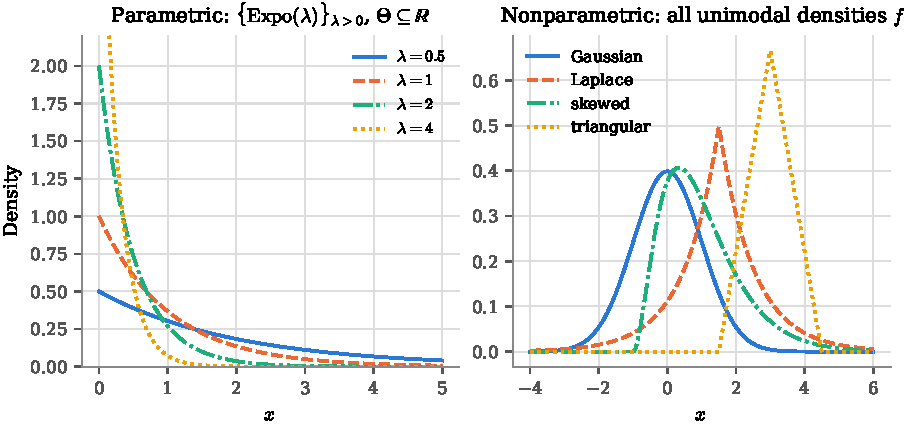
\includegraphics[width=\textwidth]{fig_parametric_vs_nonparametric}
\caption{Left: four members of the parametric family $\{\Expo(\lambda)\}_{\lambda > 0}$, at $\lambda = 0.5, 1, 2, 4$. Right: four members of the nonparametric family of all unimodal densities: Gaussian, Laplace, a skewed density and a triangular one.}
\label{fig:paramnonparam}
\end{figure}

A third kind: if $\Theta = \Theta_1 \times \Theta_2$ where $\Theta_1$ is finite-dimensional and $\Theta_2$ is infinite-dimensional, the model is \textbf{semiparametric}.
In these models you only care to estimate the finite-dimensional parameter, and the infinite-dimensional one is called a \textbf{nuisance parameter}.
The standard example is the Cox proportional hazards model from survival analysis, where the conditional CDF of a survival time $Y$ given covariates $X = x$ has the form
\[
F(t) = 1 - \exp \left( - \int_0^t h(u) e^{\beta^\top x} \, \mathrm{d}u \right),
\]
with $h$ an unknown non-negative nuisance function and $\beta \in \real^d$ the parameter of interest.
This book does not develop such models; the example is here so that you have seen what a semiparametric parameter space looks like, with $\Theta_1 = \real^d$ for $\beta$ and $\Theta_2$ the space of non-negative functions $h$.

\begin{bridge}[the regression conditions as a model]
An introductory course checks four conditions, sometimes remembered as LINE, before any inference about a regression slope: the mean of $y$ is a linear function of $x$, and the errors are independent, normal and of equal variance at every $x$.
Together they are one parametric model, with the $x_i$ treated as fixed: L is the line in $Y_i = \beta_0 + \beta_1 x_i + \epsilon_i$, and I, N and E together say $\epsilon_1, \ldots, \epsilon_n \iid \Gauss(0, \sigma^2)$, so the parameter is $(\beta_0, \beta_1, \sigma^2) \in \real^2 \times (0, \infty)$.
Replace N by `the errors are i.i.d.\ from some distribution with mean $0$ and finite variance' and the model is semiparametric: $(\beta_0, \beta_1)$ is the parameter of interest and the error distribution is an infinite-dimensional nuisance parameter.
Least squares still estimates the line without bias in that model; what N adds is the exact $t$ distribution of the slope's $t$ statistic, as it does for the $t$-test of a mean (\cref{ch:t-test}).
\end{bridge}

\section{Identifiability}
\label{sec:models-identifiability}

The first thing to ask of a model is whether it's well-specified.
You can't verify it, since the true $\Pr$ is exactly what you don't know, but you can ask whether it's plausible, and the mathematics that follows assumes it.
If it isn't, $\theta^*$ doesn't exist and `estimating the true parameter' has no meaning; what the estimators of Part IV estimate in that case is the subject of \cref{ch:distances}.
Presuming your model is well-specified, you also need to ascertain whether the parameter of the model is \textit{identifiable}.
Identifiability is a property of the parameterization: of the map from $\Theta$ to the family, not of the family itself, and not of any estimator or estimation procedure.

\begin{definition}[Identifiability]
\label{def:identifiable}
The parameter $\theta \in \Theta$ is \textbf{identifiable} if the map $\theta \mapsto \Pr_{\theta}$ is injective (one-to-one, \toolkit{sec:math-maps}).
That is:
\[
\theta_1 \neq \theta_2 \implies \Pr_{\theta_1} \neq \Pr_{\theta_2},
\]
or equivalently, taking the contrapositive:
\[
\Pr_{\theta_1} = \Pr_{\theta_2} \implies \theta_1 = \theta_2.
\]
\end{definition}

\begin{inwords}
\textbf{In words.} Different labels, different distributions. Then knowing the distribution (which is what infinitely many data would tell you) pins down the label.
\par\smallskip
\textbf{For the kiss data.} $p_1 \neq p_2$ gives $\Bern(p_1) \neq \Bern(p_2)$, since the two put different probabilities on $1$; $p$ is identifiable. The example below shows a model where two different labels give the same distribution.
\end{inwords}

\begin{center}
\begin{tikzpicture}[font=\small, >={Latex[length=2mm]}]
  \begin{scope}
    \node[font=\scriptsize] at (0.5,2.6) {$\Theta$};
    \node[font=\scriptsize] at (3.3,2.6) {distributions};
    \foreach \y/\l in {2.0/$\theta_1$, 1.3/$\theta_2$, 0.6/$\theta_3$} { \fill (0.5,\y) circle (1.8pt); \node[left=1pt, font=\scriptsize] at (0.5,\y) {\l}; }
    \foreach \y/\l in {2.0/$\Pr_{\theta_1}$, 1.3/$\Pr_{\theta_2}$, 0.6/$\Pr_{\theta_3}$} { \fill (3.3,\y) circle (1.8pt); \node[right=1pt, font=\scriptsize] at (3.3,\y) {\l}; }
    \foreach \y in {2.0, 1.3, 0.6} \draw[->, boxaqua!70!black] (0.6,\y) -- (3.2,\y);
    \node[below, font=\scriptsize] at (1.9,0.2) {identifiable: one-to-one};
  \end{scope}
  \begin{scope}[xshift=6.2cm]
    \node[font=\scriptsize] at (0.5,2.6) {$\Theta$};
    \node[font=\scriptsize] at (3.3,2.6) {distributions};
    \foreach \y/\l in {2.0/$\theta_1$, 1.3/$\theta_2$, 0.6/$\theta_3$} { \fill (0.5,\y) circle (1.8pt); \node[left=1pt, font=\scriptsize] at (0.5,\y) {\l}; }
    \foreach \y/\l in {1.65/$\Pr_{\theta_1} = \Pr_{\theta_2}$, 0.6/$\Pr_{\theta_3}$} { \fill (3.3,\y) circle (1.8pt); \node[right=1pt, font=\scriptsize] at (3.3,\y) {\l}; }
    \draw[->, boxorange!80!black] (0.6,2.0) -- (3.2,1.68);
    \draw[->, boxorange!80!black] (0.6,1.3) -- (3.2,1.62);
    \draw[->, boxaqua!70!black] (0.6,0.6) -- (3.2,0.6);
    \node[below, font=\scriptsize] at (1.9,0.2) {not identifiable: two parameters, one distribution};
  \end{scope}
\end{tikzpicture}
\end{center}

This definition means that distinct values of $\theta$ should correspond to distinct probability distributions.
Intuitively, if the parameter $\theta$ is identifiable you can go from $\Pr_{\theta}$ to $\theta$.
But if $\theta$ is \textit{not} identifiable you can have multiple $\theta$'s that give the same $\Pr$.
This means that even if you had an infinite number of observations, so that you knew $\Pr$ exactly, you'd have no way of deciding which of those $\theta$'s produced it.

Alternatively, think of it this way: if you are handed $\Pr_\theta$, can you actually recover $\theta$?
If not, if $\theta$ is not identifiable, then there are multiple $\theta$ that yield the distribution you were handed.
So if you're going to use the parameter to learn about a distribution, then you must make sure the parameter is identifiable.
Data can only ever tell you about $\Pr$; identifiability is what lets you translate that into a statement about $\theta$.

The formal way of convincing someone that the parameter is \textit{not} identifiable is to exhibit two different parameter values that give the same distribution, as the next example shows.

\subsection{Example: a non-identifiable parameter}

\begin{example}
\label{ex:nonidentifiable}
Let $X_i = \ind(Y_i \geq 0)$ for i.i.d.\ r.v.s $Y_1, \ldots, Y_n \sim \Gauss(\mu, \sigma^2)$, where $\mu$ and $\sigma^2$ are unknown and the $Y_i$ are \textit{not observed}; you only see whether each one is non-negative.
Then $\mu$ and $\sigma^2$ are \textit{not} identifiable from the common distribution of the $X_i$'s.
\end{example}

To see why, first note that, by definition, the $X_i$ are Bernoulli r.v.s since the indicator function $\ind(Y_i \geq 0)$ simply tells you if $Y_i$ is non-negative or not and assigns 1 or 0 accordingly.
So you want to determine whether you can find $\mu$ and $\sigma^2$ just from observing the Bernoulli r.v.s $X_i$.

Now, as the $X_i$'s are Bernoulli, what is the relevant parameter?
It's the probability that $Y \geq 0$, so that $X_i \sim \Bern(\Pr(Y \geq 0))$, where $Y$ represents any one of the $n$ i.i.d.\ r.v.s $Y_i$.
Because $Y$ is a non-standard Gaussian r.v., standardize it to get:
\[
\Pr(Y \geq 0) = \Pr \left( \frac{Y - \mu}{\sigma} \geq -\frac{\mu}{\sigma} \right) = 1 - \Phi \left( -\frac{\mu}{\sigma} \right) = \Phi \left( \frac{\mu}{\sigma} \right).
\]
So the parameter of this Bernoulli is $p = \Phi(\mu/\sigma)$.
As $\Phi$ is invertible, you can solve for $\mu/\sigma$ to get:
\[
\frac{\mu}{\sigma} = \Phi^{-1}(p).
\]
So you can learn $p$ (it's a Bernoulli proportion), apply $\Phi^{-1}$, and this gives you $\mu/\sigma$.
Hence the ratio $\mu/\sigma$ is identifiable.

However, $\mu$ and $\sigma^2$ by themselves are \textit{not} identifiable.
Why?
One way to see it is to count dimensions.
The parameter of a Bernoulli r.v.\ is one number between 0 and 1.
The parameter of the Gaussian is two numbers, $\mu$ and $\sigma^2$.
A continuous map from a two-dimensional space onto a one-dimensional one can't be one-to-one: it has to send whole curves of $(\mu, \sigma^2)$ pairs to the same $p$.

But the formal way mentioned above requires a counterexample.
So, let $(\mu_1, \sigma^2_1) = (1,4)$ and $(\mu_2, \sigma^2_2) = (2,16)$.
Then:
\[
\frac{\mu_1}{\sqrt{\sigma^2_1}} = \frac{1}{\sqrt{4}} = \frac{1}{2}, \,\, \text{ and } \,\, \frac{\mu_2}{\sqrt{\sigma^2_2}} = \frac{2}{\sqrt{16}} = \frac{1}{2}.
\]
Hence different parameter vectors, $(1,4)$ and $(2,16)$, both yield the same Bernoulli parameter $p = \Phi(1/2) = 0.691$, so $\Pr_{(1,4)} = \Pr_{(2,16)}$ while $(1,4) \neq (2,16)$.
\Cref{fig:identifiability} shows the two Gaussians, which look nothing alike, putting the same mass above zero, and shows in the parameter space what the counterexample is a sample of: a whole ray of parameters producing one distribution.
On the left, $\Gauss(1, 4)$ and $\Gauss(2, 16)$ are different distributions, but the only thing you observe is whether $Y \geq 0$, and both put probability $\Phi(1/2) = 0.691$ there.
On the right, in the $(\mu, \sigma)$ plane, every point on the orange ray $\mu/\sigma = 1/2$ produces that same Bernoulli, and every other ray produces some other one.
The observable distribution identifies the ray, that is, $\mu/\sigma$, and nothing more; the counterexample above is two points on the orange ray.

\begin{figure}[htbp]
\centering
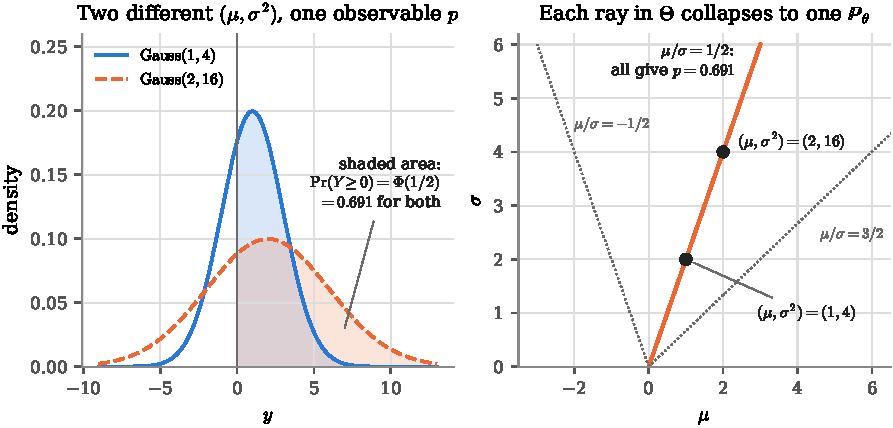
\includegraphics[width=\textwidth]{fig_identifiability}
\caption{\Cref{ex:nonidentifiable}. Left: the densities of $\Gauss(1, 4)$ and $\Gauss(2, 16)$, each with its mass above zero shaded. Right: the $(\mu, \sigma)$ plane, with the ray $\mu/\sigma = 1/2$ in orange, the counterexample's two points marked, and two other rays dotted.}
\label{fig:identifiability}
\end{figure}

\subsection{More examples}

Three variations are worth doing in your head because the pattern is always the same: write down the distribution of what you actually observe as a function of $\theta$, and ask whether that function is one-to-one.

\begin{example}[Censored Exponential]
\label{ex:censored-expo}
Let $X \sim \Expo(\lambda)$ with $\lambda > 0$ unknown, and suppose you observe only $Y = \ind(X > 5)$, a censored version of $X$: you can't see $X$, only whether it exceeded $5$.
Then $Y \sim \Bern(f(\lambda))$ with $f(\lambda) = \Pr(X > 5) = \int_5^\infty \lambda e^{-\lambda x} \, \mathrm{d}x = e^{-5\lambda}$.
The model for $Y$ is $\left( \{0,1\}, (\Bern(e^{-5\lambda}))_{\lambda > 0} \right)$, and $\lambda$ \textit{is} identifiable because $\lambda \mapsto e^{-5\lambda}$ is strictly decreasing, hence injective: from $p = \Pr(Y = 1)$ you recover $\lambda = -\ln(p)/5$.
Censoring loses information (you'll estimate $\lambda$ less precisely than from the $X$'s), but it doesn't lose identifiability.
Compare \cref{ex:nonidentifiable}, where the trouble was not the censoring but the two-dimensional parameter behind a one-dimensional observable.
\end{example}

\begin{example}[Squaring a uniform]
Let $X_i = Y_i^2$ where $Y_1, \ldots, Y_n \iid \text{Unif}([0, a])$ are unobserved.
Is $a$ identifiable?
Yes: $X_i$ takes values in $[0, a^2]$, and $\Pr(X_i \leq x) = \Pr(Y_i \leq \sqrt{x}) = \sqrt{x}/a$ for $0 \leq x \leq a^2$.
Different $a$ give different CDFs (for instance, different supports), so the map $a \mapsto \Pr_a$ is injective.
\end{example}

\begin{example}[Thresholding a uniform at half its range]
Let $X_i = \ind(Y_i \geq a/2)$ where $Y_1, \ldots, Y_n \iid \text{Unif}([0, a])$ are unobserved.
Is $a$ identifiable?
No: $\Pr(Y_i \geq a/2) = 1/2$ for \textit{every} $a > 0$, so $X_i \sim \Bern(1/2)$ whatever $a$ is.
The map $a \mapsto \Pr_a$ is constant, the worst possible failure of injectivity: the data carry no information about $a$ at all.
\end{example}

\Cref{fig:identmaps} draws the three maps side by side; identifiability is the shape of the curve.
In each example the observation is a Bernoulli whose parameter $p$ is a function of $\theta$.
On the left, the censored Exponential has $p = e^{-5\lambda}$, strictly decreasing, so each $p$ comes from exactly one $\lambda$.
In the middle, the uniform thresholded at half its range has $p = \frac12$ for every $a$, so the observation says nothing about $a$.
On the right, the Gaussian sign example has $p = \Phi(\mu/\sigma)$, drawn against $\mu$ for three values of $\sigma$: one value of $p$ is reached by a whole ray of $(\mu, \sigma)$ pairs, the ray of \cref{fig:identifiability}.
Identifiable means the curve never takes the same value twice.

\begin{figure}[htbp]
\centering
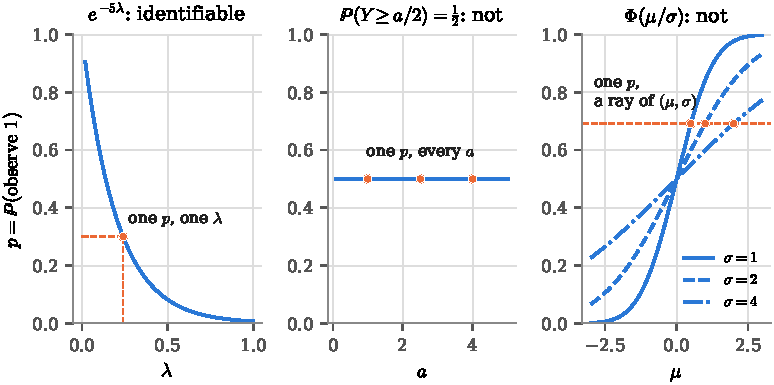
\includegraphics[width=\textwidth]{fig_identifiable_maps}
\caption{The observable Bernoulli parameter $p$ as a function of $\theta$. Left: the censored Exponential, $p = e^{-5\lambda}$. Middle: the uniform thresholded at half its range, $p = \frac12$. Right: the Gaussian sign example, $p = \Phi(\mu/\sigma)$ against $\mu$, one line style per $\sigma$.}
\label{fig:identmaps}
\end{figure}

\begin{bridge}[collinearity, a non-identifiability you have already met]
In a regression course, if two predictors are perfectly collinear (say $x_2 = 2x_1$), the software drops one of them or leaves its coefficient blank.
That is non-identifiability.
The model $Y = \beta_1 x_1 + \beta_2 x_2 + \epsilon$ with $x_2 = 2x_1$ produces exactly the same distribution of $Y$ for every $(\beta_1, \beta_2)$ with the same value of $\beta_1 + 2\beta_2$: a whole line of parameter vectors, one distribution, exactly like the ray in \cref{fig:identifiability}.
The data can tell you $\beta_1 + 2\beta_2$ and nothing more, and no sample size fixes it.
Dropping a predictor is the software's way of choosing one point on the line.
\Cref{ch:regression-multi} returns to this when it needs the design matrix to have full rank.
\end{bridge}

\section{Gaussian mixture models}
\label{sec:models-gmm}

A mixture of Gaussians is best described in terms of the generative model.
You first generate a discrete variable that determines which of the component Gaussians to use, and then generate an observation from that chosen Gaussian density.

More formally, suppose you have two Gaussian r.v.s, $X^{(1)}$ and $X^{(2)}$, such that $X^{(1)} \sim \Gauss(\mu_1, \sigma^2_1)$ and $X^{(2)} \sim \Gauss(\mu_2, \sigma^2_2)$.
Their PDFs are:
\begin{align*}
f_1(x) &= \frac{1}{\sigma_1 \sqrt{2 \pi}} \exp \left( - \frac{(x-\mu_1)^2}{2 \sigma_1^2} \right), \\
f_2(x) &= \frac{1}{\sigma_2 \sqrt{2 \pi}} \exp \left( - \frac{(x-\mu_2)^2}{2 \sigma_2^2} \right).
\end{align*}
Let $\pi \in (0, 1)$ be the \textit{mixture weight}.
A \textbf{mixture} of the two Gaussians has the PDF:
\begin{align*}
f(x) &= \pi f_1(x) + (1 - \pi) f_2(x) \\
	&= \pi \left( \frac{1}{\sigma_1 \sqrt{2 \pi}} \right) \exp \left( - \frac{(x-\mu_1)^2}{2 \sigma_1^2} \right)  + (1-\pi) \left( \frac{1}{\sigma_2 \sqrt{2 \pi}} \right) \exp \left( - \frac{(x-\mu_2)^2}{2 \sigma_2^2} \right).
\end{align*}
(The symbol $\pi$ does double duty here, as the weight and as the constant $3.14159\ldots$ inside the normalizing constants; both uses are standard and the context always tells them apart.)

To better understand a mixture of Gaussian distributions, think of it as a latent variable model.\footnote{Recall that a latent variable is an unobserved variable that can only be inferred indirectly from observable variables.}
Proceed in 3 steps:
\begin{enumerate}
\item \textbf{Latent component selection:} Sample $Z \sim \Bern(\pi)$, so $Z = 1$ with probability $\pi$ and $Z = 0$ with probability $1 - \pi$.
\item \textbf{Independent sampling:} Sample $X^{(1)} \sim \Gauss(\mu_1, \sigma_1^2)$ and $X^{(2)} \sim \Gauss(\mu_2, \sigma_2^2)$, independent of $Z$ and of each other.
Both values are conceptually sampled regardless of $Z$'s value.
\item \textbf{Mixture realization:} Define the r.v.\ $X$ by:
\[
X = Z X^{(1)} + (1 - Z) X^{(2)}.
\]
Only one of the two is used: $X = X^{(1)}$ if $Z = 1$ and $X = X^{(2)}$ if $Z = 0$.
\end{enumerate}

\textbf{Question:} How can this be a \textit{mixture} if each sample comes from exactly \textit{one} Gaussian?

\textbf{Answer:} The answer lies in distinguishing between:
\begin{itemize}[nosep]
\item \textbf{Sample generation}: Each individual observation is generated from only one component, determined by $Z$.
\item \textbf{Distribution properties}: The overall probability distribution of $X$ is a weighted mixture of both Gaussians because you don't get to see $Z$.
\end{itemize}
Mathematically, for any possible value $x$, the law of total probability over $Z$ gives the density
\[
f(x) = \Pr(Z = 1) f_1(x) + \Pr(Z = 0) f_2(x) = \pi f_1(x) + (1-\pi) f_2(x),
\]
so both components contribute to the overall distribution, weighted by their probabilities.
From the population perspective, if you generate $n$ samples from this model, approximately $n\pi$ of them come from $\Gauss(\mu_1, \sigma_1^2)$ and approximately $n(1 - \pi)$ from $\Gauss(\mu_2, \sigma_2^2)$.
\Cref{fig:gmm} shows both perspectives.
On the left, the mixture density is the sum of the two weighted components.
On the right, each of the $400$ draws came from exactly one component, and its color records which; the black mixture density over the histogram is what you see when you cannot tell.

\begin{figure}[htbp]
\centering
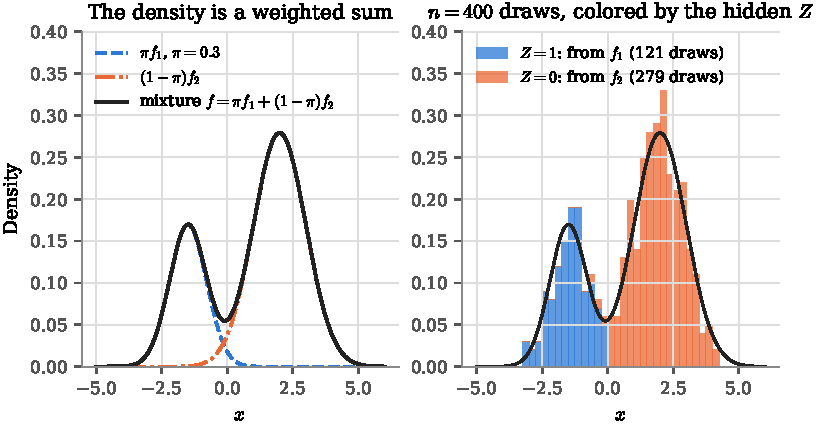
\includegraphics[width=\textwidth]{fig_gaussian_mixture}
\caption{A two-component Gaussian mixture with $\pi = 0.3$, $\Gauss(-1.5, 0.5)$ (blue) and $\Gauss(2, 1)$ (orange). Left: the two weighted components and their sum, the mixture density (black). Right: $400$ draws, histogrammed and colored by the latent $Z$, with the mixture density over them.}
\label{fig:gmm}
\end{figure}

An alternative specification of the same r.v.\ is $X = (X^{(1)})^Z (X^{(2)})^{1-Z}$, which picks the same component as before.
The latent variable perspective is especially useful for inference algorithms like EM (expectation-maximization), where you need to estimate both the component parameters $(\mu_1, \sigma_1^2, \mu_2, \sigma_2^2)$ and the mixture weight $\pi$ without ever observing which component produced which observation.

\begin{bridge}[a histogram with two peaks]
An introductory course reads a histogram with two peaks as a sign that the data may mix two groups, and suggests separating them if some variable records the group.
The Gaussian mixture is that reading as a model, for when no variable does: $Z$ is the unrecorded group, each component is the distribution within one group, and $\pi$ is the share of the first group.
With the groups recorded, $\pi$ would be estimated by the proportion of observations in the first group, a sample proportion like $\hat{p}$, and each component from its own group's mean and variance.
Without them, \cref{sec:lik-em} estimates all five parameters at once; for the waiting times between eruptions of the Old Faithful geyser, with peaks near $55$ and $80$ minutes, it puts about a third of the waits in the short group.
\end{bridge}

\subsection{Possible Gaussian mixture models}

There are several scenarios for a model with mixtures of Gaussians, depending on the constraints imposed on its 5 parameters.
Here are 3 possible examples.
It should be noted that, for clarity but with an abuse of notation, the PDFs of the two Gaussian r.v.s are not explicitly written below; each distribution is written generically as $\Gauss(\mu_1, \sigma_1^2)$.
\begin{enumerate}
\item Model where all 5 parameters are unknown:
\[
\left( \real, (\pi \cdot \Gauss(\mu_1, \sigma_1^2) + (1-\pi) \cdot \Gauss(\mu_2, \sigma_2^2))_{\pi \in (0,1), \, \mu_1, \mu_2 \in \real, \, \sigma_1^2, \sigma_2^2 \in (0,\infty)} \right).
\]
\item Model with known variances, and for simplicity suppose $\sigma_1^2 = \sigma_2^2 = 1$:
\[
\left( \real, (\pi \cdot \Gauss(\mu_1, 1) + (1-\pi) \cdot \Gauss(\mu_2, 1))_{\pi \in (0,1), \, \mu_1, \mu_2 \in \real} \right).
\]
\item Model with only unknown means, and for simplicity suppose $\sigma_1^2 = \sigma_2^2 = 1$ and $\pi = 1/2$:
\[
\left( \real, \left( \tfrac{1}{2} \cdot \Gauss(\mu_1, 1) + \tfrac{1}{2} \cdot \Gauss(\mu_2, 1) \right)_{\mu_1, \mu_2 \in \real} \right).
\]
\end{enumerate}

\begin{pitfall}[mixtures are identifiable only up to relabeling]
Take the third model and the two parameter vectors $(\mu_1, \mu_2) = (-1, 2)$ and $(\mu_1, \mu_2) = (2, -1)$.
They're different points of $\Theta = \real^2$, and they give exactly the same density: $\frac12 f_{-1} + \frac12 f_{2} = \frac12 f_{2} + \frac12 f_{-1}$.
So by \cref{def:identifiable} the parameter is not identifiable; the same happens in the first two models with $(\pi, \mu_1, \sigma_1^2, \mu_2, \sigma_2^2) \leftrightarrow (1-\pi, \mu_2, \sigma_2^2, \mu_1, \sigma_1^2)$.
This failure is called \textit{label switching}, and it's harmless in a way \cref{ex:nonidentifiable} is not: the two parameter vectors describe the same two components with their names swapped, so the data do pin down the components, just not which one is `first'.
The fix is a convention such as $\mu_1 < \mu_2$, which restricts $\Theta$ to half the plane and removes the swap; that nothing else collides, so that the map is then injective, is a theorem about finite Gaussian mixtures that is not proved here.
The lesson is that non-identifiability is sometimes a defect of the labeling rather than of the information in the data, and the first thing to ask when you find it is which of the two you're looking at.
\end{pitfall}

\section{What comes next}
\label{sec:models-next}

A model fixes the family of candidate distributions.
Three things are done inside it, and they are Part III: guess $\theta$ (\cref{ch:estimators}), attach a range to the guess (\cref{ch:confidence-intervals}), and decide a yes/no question about $\theta$ (\cref{ch:tests-foundations}).
All three are stated for a general model $(E, (\Pr_\theta)_{\theta \in \Theta})$ and computed, as always, for the kiss model.
All three also rest on what an average of $n$ draws does as $n$ grows, and that is Part II, which comes first: where the average settles (\cref{ch:lln}), how it fluctuates on the way (\cref{ch:clt}), what may be done to those limits (\cref{ch:limit-tools}), and the Gaussian distribution the limits land on (\cref{ch:gaussian}).

\section{Summary}
\label{sec:models-summary}

\begin{itemize}[nosep]
\item A statistical model is $\left( E, (\Pr_\theta)_{\theta \in \Theta} \right)$: a sample space and a family of candidate distributions for $X$, indexed by a parameter. Parameters define distributions; learning one is learning the other. The sample space must not depend on $\theta$.
\item Assumptions buy fewer parameters: the siblings PMF has six, the shifted Poisson one. The price is misspecification if the assumption is wrong.
\item Three layers: the sample space $\Omega$ (every complete outcome), random variables (functions on $\Omega$, the measuring instruments and the rules applied to their readings), and the observations (those functions evaluated at the one outcome that happened). An estimate is one draw from the estimator's distribution. Inference does not invert the chain; it holds the one value up against the distribution of the rule. For fixed $n$, take $\Omega = E^n$.
\item Well-specified: the true $\Pr$ is some $\Pr_{\theta^*}$ in the family. Everything from Part III on assumes this; \cref{ch:distances} says what estimators estimate when it fails.
\item Parametric: $\Theta \subseteq \real^d$. Nonparametric: $\Theta$ is a space of functions. Semiparametric: a finite-dimensional parameter of interest plus an infinite-dimensional nuisance parameter.
\item Identifiable: $\theta \mapsto \Pr_\theta$ is injective, so knowing the distribution of the data would tell you $\theta$. To show a parameter is not identifiable, exhibit two parameter values with the same distribution. Observing only a function of the data can destroy identifiability (two numbers behind one observable proportion) or leave it intact (one number behind one proportion, injectively); what matters is whether the map from the parameter to the observable distribution is one-to-one.
\item A Gaussian mixture is a latent-variable model: pick a component with $Z \sim \Bern(\pi)$, then draw from it. Its density is $\pi f_1 + (1-\pi) f_2$. Its parameter is identifiable only up to swapping the component labels.
\end{itemize}

\section{Exercises}
\label{sec:models-exercises}

\begin{exercise}
Which of the following is a statistical model? (1) $\left( \{1\}, (\Bern(p))_{p \in (0,1)} \right)$; (2) $\left( \{0,1\}, (\Bern(p))_{p \in (0.2, 0.4)} \right)$; (3) both; (4) neither.
\end{exercise}
\begin{solution}
(2). The first has a sample space that excludes the outcome $0$, which every $\Bern(p)$ puts mass on. The second is a legitimate model with a restricted parameter space; whether it's well-specified is a separate question.
\end{solution}

\begin{exercise}
Let $\Xton \iid \text{Unif}([0, a])$ for some unknown $a > 0$. Which is the associated statistical model: (1) $\left( [0, a], (\text{Unif}([0,a]))_{a > 0} \right)$; (2) $\left( \real_+, (\text{Unif}([0,a]))_{a > 0} \right)$; (3) $\left( \real, (\text{Unif}([0,a]))_{a > 0} \right)$; (4) none?
\end{exercise}
\begin{solution}
The intended answer is (2), and (1) is the one that is definitely wrong: the sample space can't depend on the unknown $a$. Both $\real_+$ and $\real$ contain every observation for every $a$, so by \cref{def:statmodel} (3) is a legitimate model too; the convention is to take $E = \real_+$, the smallest natural set that works, and that convention is what the question is testing.
\end{solution}

\begin{exercise}
Which of these models are parametric? (A) $E = \{0, 1, 2, \ldots\}$ and $\{\Pr_\theta\}$ is the set of all distributions on $E$. (B) $E = \{0,1\}$, $(\Bern(\theta))_{\theta \in [0,1]}$. (C) $E = \real$, $(\Gauss(0, \sigma^2))_{\sigma^2 > 0}$. (D) $E = \{1,2,3,4\}$ and $\Pr_{(p_1, \ldots, p_4)}$ puts probability $p_i$ on $i$, with $p_i \geq 0$ and $\sum p_i = 1$. (E) $E = \real$, $(\Gauss(\mu, \sigma^2))_{\mu \in \real, \sigma^2 > 0}$. (F) $E = [0, \infty)$, $(\text{Unif}([0, \theta]))_{\theta > 0}$. (G) $E = [0,1]$ and $\{\Pr_f\}$ is the set of all distributions with a continuous density $f$ on $[0,1]$.
\end{exercise}
\begin{solution}
B, C, D, E, F. In (A) a member of the family needs infinitely many numbers (a probability for every non-negative integer). (B), (C), (F) need one number, (E) two, (D) three (the fourth $p_i$ is determined by the other three). In (G) a member is a continuous function on $[0,1]$, which no finite list of numbers specifies.
\end{solution}

\begin{exercise}
You observe $X_i = \ind(Y_i \geq c)$ for $Y_i \iid \Gauss(\mu, 1)$ with $\sigma^2 = 1$ known and $c$ a known constant. Is $\mu$ identifiable? What if instead $\sigma^2$ is unknown and $\mu = 0$ is known?
\end{exercise}
\begin{solution}
$\Pr(Y_i \geq c) = 1 - \Phi(c - \mu) = \Phi(\mu - c)$, strictly increasing in $\mu$, so $\mu$ is identifiable: $\mu = c + \Phi^{-1}(p)$. With $\mu = 0$ known and $\sigma$ unknown, $\Pr(Y_i \geq c) = \Phi(-c/\sigma)$: for $c \neq 0$ this is strictly monotone in $\sigma$ and $\sigma$ is identifiable; for $c = 0$ it equals $1/2$ for every $\sigma$, and $\sigma$ is not. The threshold matters: thresholding at the known mean throws away all information about the spread, as in the uniform example.
\end{solution}

\begin{exercise}
In the two-component mixture with all five parameters unknown, is the parameter $(\pi, \mu_1, \sigma_1^2, \mu_2, \sigma_2^2)$ identifiable on the restricted parameter space where $\mu_1 < \mu_2$? What about the point $\pi = 1$, if it were allowed?
\end{exercise}
\begin{solution}
Ordering the means removes the label-switching ambiguity, and it's a theorem (not proved here) that finite Gaussian mixtures are then identifiable. The endpoint $\pi = 1$ is excluded from $\Theta$ for a good reason: at $\pi = 1$ the density is $f_1$ whatever $(\mu_2, \sigma_2^2)$ are, so every value of the second component's parameters gives the same distribution. A component with zero weight is invisible, which is why the weight is required to be in the open interval $(0, 1)$.
\end{solution}
